
\begin{figure}[h!]
\textbf{Tema d'Esame di Gennaio 2016}\\ \\
Una molla viene compressa di 17 cm prima di lanciare una palla verso un piano inclinato
senza attrito. La palla ha massa 1kg e il piano inclinato ha un'altezza H=1.28 m. Quanto vale
la costante elastica della molla affinché la palla arrivi con una velocità di 4 m/s in cima al
piano ?
\\
	\begin{center}
		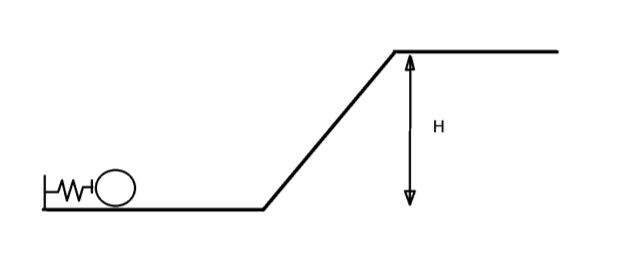
\includegraphics[scale=0.5]{ES2/GEN022016.jpg}
	\end{center}
\end{figure}

\begin{figure}[h!]
\textbf{Tema d'Esame di Febbraio 2016}\\ \\
Una palla di massa $250g$ è lanciata da una molla con costante elastica $63 N/m$ compressa di $45 cm$. La palla viaggia attraverso un piano inclinato alto $72 cm$. Una volta arrivata in cima al piano inclinato la palla incontra una superficie piatta frenante. Il coefficente d'attrito dinamico palla-superficie è di $m=0.42$. Che distanza percorre la palla sulla superficie frenante prima di fermarsi?
\\
	\begin{center}
		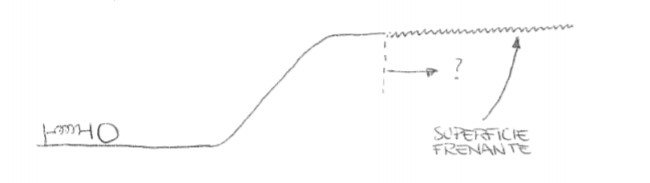
\includegraphics[scale=0.5]{ES2/FEB022016.jpg}
	\end{center}
\end{figure}

\begin{figure}[h!]
\textbf{Tema d'Esame di Giugno 2016}\\ \\
Una molla ideale può essere compressa di $1.0 m$ da una forza di $100 N$. La stessa molla è posta alla fine di un piano inclinato con attrito (coefficiente $0.2$) che forma un angolo di 30$^{\circ}$ con l'orizzontale. Una massa $M$ di $10 kg$ viene lasciata cadere da ferma dal vertice del piano inclinato e si arresta momentaneamente dopo aver compresso la molla di $2.0 m$. Qual'è la velocità della massa un attimo prima di toccare la molla? 
\\
	\begin{center}
		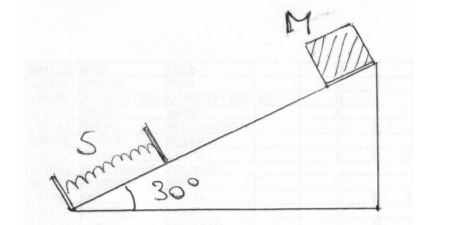
\includegraphics[scale=0.5]{ES2/GIU022016.jpg}
	\end{center}
\end{figure}

\begin{figure}[h!]
\textbf{Tema d'Esame di Luglio 2016}\\ \\
La molla della figura ha una costante elastica $k = 120 \frac{N}{m}$ e una lunghezza a riposo di $45cm$. Quando un blocco di massa $M$ viene attaccato alla molla l'estensione di equilibrio della molla è $60cm$. Il piano inclinato è liscio(senza attrito) e forma un angolo di $40^\circ$ con l'orizzontale. Se la massa viene tirata leggermente verso il basso e viene rilasciata, qual è il periodo di oscillazione? 
\\
	\begin{center}
		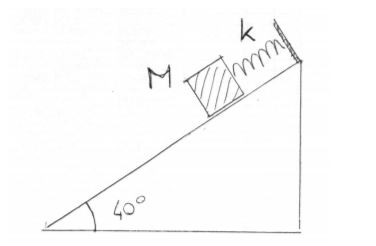
\includegraphics[scale=0.5]{ES2/LUG022016.jpg}
	\end{center}
\end{figure}

